% Define number set symbols.
\newcommand{\N}{\mathbb{N}}
\newcommand{\Z}{\mathbb{Z}}
\newcommand{\Q}{\mathbb{Q}}
\newcommand{\R}{\mathbb{R}}
\newcommand{\C}{\mathbb{C}}

\chapter{Functions and Graphs}
\section{Composite Functions}
A function $f(x) = 3x+9$ will take in any value for $x$, and substitutes it into the expression $3x+9$. If another expression would be passed into $f(x)$, such as $x-2$, then the result would be $3(x-2)+9$. A composite function is one where two functions are combined, similar to above.

Suppose $f(x) = 2x$ and $g(x) = x+1$, then composite functions $f(g(x))$ and $g(f(x))$ can be found as follows:
\begin{align*}
	f(g(x)) &= 2(x+1) & g(f(x)) &= (2x)+1\\
	&=2x+2 & &=2x+1
\end{align*}

A composite function can get tiring to write out all the time. So it could be written as $h(x)=f(g(x))$.

\subsection{Example}
$f(x)=x^2+1$ and $g(x)=\frac{1}{x} \left(x\neq0\right)$. Find $h(x)=f(g(x))$ and $h(x)=g(f(x))$.
\begin{align*}
	h(x)&=f\left(\frac{1}{x}\right) & k(x)&=g\left(x^2+1\right)\\
	&=\left(\frac{1}{x}\right)^2-2 & &=\frac{1}{x^2+1}\\
	&=\frac{1}{x^2}-1
\end{align*}


\section{Domains and Set Notation}
A function most often can't take all numbers as inputs. For example, a function of the area of a rectangle might be written as $f(x)=x^2+2x-8$. Since it's a function of real-life area in terms of lengths, the area cannot be negative. After some thinking, it can be concluded that $x$ must be 2 or larger. So the function's domain is any number larger or equal to 2.

Additionally, a real number (aka decimal number) could also be passed in to the function, but maybe that's not what you want. You can also define the domain to only include natural numbers (positive whole numbers).

Applying these two factors, the domain of the function is $\{x \in \N \mid x \geq 2\}$

Set (or rather set-builder) notation is a way of describing a set of numbers. In relation to domains, it details what set of numbers can be an acceptable input of the function. The kinds of set number symbols that exist commonly are
\begin{itemize}
	\item $\N$, natural numbers. Non-negative integers (so starting with 0, counting up in steps of 1).
	\item $\Z$, integers. Any number that can be written without a fractional component (``whole" numbers).
	\item $\Q$, rational numbers. A number which can be written as a fraction with an integer numerator and a non-zero natural denominator\footnote{Negative denominators can exist, but are avoided, as they can be expressed as a negative numerator instead.}.
	\item $\R$, real numbers. Any number that can be represented on a number line.
\end{itemize}

\subsection{Example}
Find a suitable domain for the function $\frac{1}{x^2-1}$.

\begin{equation*}
	\{x \in \R \mid x \neq \sqrt{2}\}
\end{equation*}


\section{Inverse Functions}
An inverse function ($f^{-1}(x)$) will do the opposite as what its normal counterpart ($f(x)$) does. For example,
\begin{align*}
	f(x) &= x^2\\
	f^{-1}(x)&=\sqrt{x}
\end{align*}

Functions are said to be inverse if $f\left(f^{-1}(x)\right) = f^{-1}\left(f(x)\right)=x$.

A trick for finding the inverse of a function is to do the following:
\begin{enumerate}
	\item replace $f(x)$ with $y$,
	\item change the subject of the formula for $x$,
	\item change $y$ to $x$, and $x$ to $f^{-1}(x)$.
\end{enumerate}

\subsection{Examples}
\begin{enumerate}
	\item
	\begin{align*}
		f(x)&=2x\\
		y&=2x\\
		x&=\frac{y}{2}\\
		f^{-1}(x)&=\frac{x}{2}
	\end{align*}
	\item
	\begin{align*}
		f(x)&=2x+1\\
		y&=2x+1\\
		2x&=y-1\\
		x&=\frac{1}{2}\left(y-1\right)\footnotemark\\
		f^{-1}(x)&=\frac{1}{2}\left(x-1\right)
	\end{align*}
	\footnotetext{Note that writing $x=\frac{y-1}{2}$ is correct too. That means that $f^{-1}(x)=\frac{x-1}{2}$ is a perfectly acceptable answer.}
\end{enumerate}


\section{Graph of $y=f(x)+a$ and \dots$-a$}
Given a graph $y=f(x)$, if asked to sketch $y=f(x)+a$, the graph would be moved $a$ places up; if asked to sketch $y=f(x)-a$, the graph would be moved $a$ places down.

In other words, the graph is moved $a$ places along the $y$-axis. A value of $-3$ would move the graph $-3$ places up (i.e. $3$ places down). Practically, add $a$ to all $y$-coordinates.

\subsection{Example}
In figure \ref{fig:verticalShiftExample}, the original graph $y=f(x)$ is drawn, along with $y=f(x)+3$.

\begin{figure}[h!]
	\centering
	\begin{subfigure}{0.475\linewidth}
		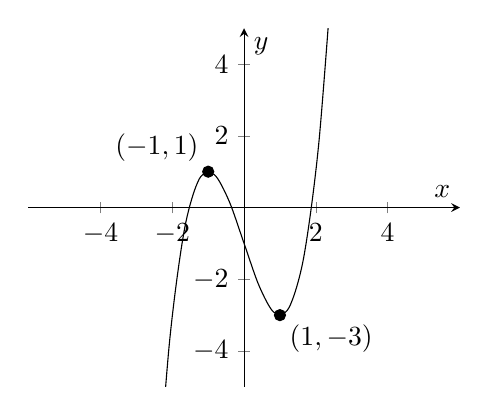
\begin{tikzpicture}[cmark/.style={label={[anchor=center]:\pgfuseplotmark{#1}}}]
			\begin{axis}
			[
				restrict y to domain=-10:10,
				restrict x to domain=-5:5,
				xlabel=$x$,
				ylabel=$y$,
				xmin=-5,
				xmax=5,
				xtick={-4,-2,...,4},
				ymin=-5,
				ymax=5,
				ytick={-4,-2,...,3},
				axis lines=center,
				axis equal,
				smooth,
				scale=0.8
			]
			\addplot [] {x^3-3*x-1};
			\coordinate
			[
				label=above left:{$(-1,1)$},
				black,
				cmark=*,
			] (a) at (-1,1);
			\coordinate
			[
				label=below right:{$(1,-3)$},
				black,
				cmark=*,
			] (a) at (1,-3);
			\end{axis}
		\end{tikzpicture}
		\caption{Some function $y=f(x)$ with a couple of given coordinates.}
	\end{subfigure}
	\begin{subfigure}{0.475\linewidth}
		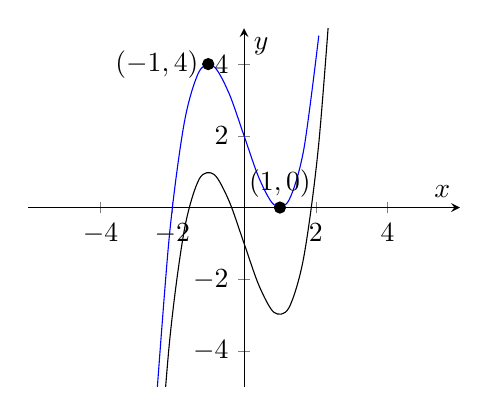
\begin{tikzpicture}[cmark/.style={label={[anchor=center]:\pgfuseplotmark{#1}}}]
			\begin{axis}
			[
				restrict y to domain=-10:10,
				restrict x to domain=-5:5,
				xlabel=$x$,
				ylabel=$y$,
				xmin=-5,
				xmax=5,
				xtick={-4,-2,...,4},
				ymin=-5,
				ymax=5,
				ytick={-4,-2,...,3},
				axis lines=center,
				axis equal,
				smooth,
				scale=0.8
			]
			\addplot [mark=none] {x^3-3*x-1};
			\addplot [color=blue,mark=none] {x^3-3*x+2};
			\coordinate
			[
				label=left:{$(-1,4)$},
				black,
				cmark=*,
			] (a) at (-1,4);
			\coordinate
			[
				label=above:{$(1,0)$},
				black,
				cmark=*,
			] (a) at (1,0);
			\end{axis}
		\end{tikzpicture}
		\caption{$y=f(x)+3$ in blue, along with the original graph.}
	\end{subfigure}
	\caption{An example of a typical question about $y=f(x)+a$ with the solution.}
	\label{fig:verticalShiftExample}
\end{figure}

To find out the transformed coordinates, add $a$ to the $y$-coordinates:
\begin{align*}
f(x)&=(-1,1) & f(x)&=(1,-3)\\
f(x)+3&=(-1,4) & f(x)+3&=(1,0)
\end{align*}


\section{Graph of $y=f(x+a)$ and \dots$-a)$}
When the $a$ is inside the bracket, it moves the graph from side to side. A graph of $y=f(x+a)$ will move the graph $a$ places \textit{left}, and $y=f(x-a)$ would move $a$ places \textit{right}.

In other words, the graph is moved $-a$ places along the $x$-axis. A value of $-3$ would move the graph 3 places to the right. Practically, add $-a$ to all $x$-coordinates. The thing to throw you off is that it is $-a$, and not $a$ that is being moved.

\subsection{Example}
The figure \ref{fig:horizontalShiftExample} is the graph $y=f(x)$ and $y=f(x+5)$.

\begin{figure}[h!]
	\centering
	\begin{subfigure}{0.475\linewidth}
		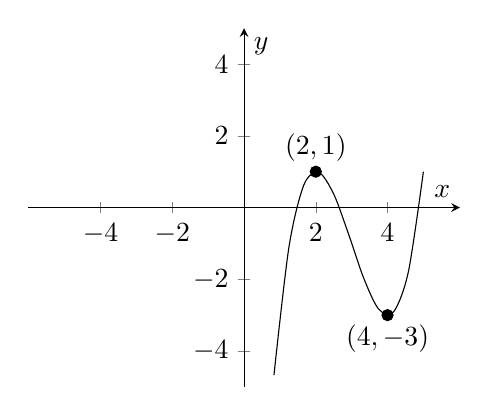
\begin{tikzpicture}[cmark/.style={label={[anchor=center]:\pgfuseplotmark{#1}}}]
		\begin{axis}
			[
				restrict y to domain=-10:10,
				restrict x to domain=-5:5,
				xlabel=$x$,
				ylabel=$y$,
				xmin=-5,
				xmax=5,
				xtick={-4,-2,...,4},
				ymin=-5,
				ymax=5,
				ytick={-4,-2,...,3},
				axis lines=center,
				axis equal,
				smooth,
				scale=0.8
			]
			\addplot [] {(x-3)^3-3*x+8};
			\coordinate
			[
				label=above:{$(2,1)$},
				black,
				cmark=*,
			] (a) at (2,1);
			\coordinate
			[
				label=below:{$(4,-3)$},
				black,
				cmark=*,
			] (a) at (4,-3);
		\end{axis}
		\end{tikzpicture}
		\caption{Some function $y=f(x)$ with a couple of given coordinates.}
	\end{subfigure}
	\begin{subfigure}{0.475\linewidth}
		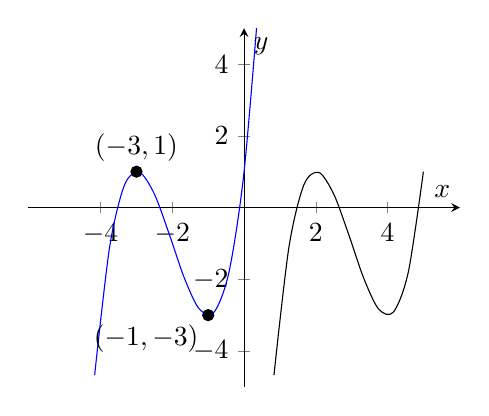
\begin{tikzpicture}[cmark/.style={label={[anchor=center]:\pgfuseplotmark{#1}}}]
			\begin{axis}
			[
				restrict y to domain=-10:10,
				restrict x to domain=-5:5,
				xlabel=$x$,
				ylabel=$y$,
				xmin=-5,
				xmax=5,
				xtick={-4,-2,...,4},
				ymin=-5,
				ymax=5,
				ytick={-4,-2,...,3},
				axis lines=center,
				axis equal,
				smooth,
				scale=0.8
			]
			\addplot [mark=none] {(x-3)^3-3*x+8};
			\addplot [color=blue,mark=none] {(x+2)^3-3*(x+5)+8};
			\coordinate
			[
				label=above:{$(-3,1)$},
				black,
				cmark=*,
			] (a) at (-3,1);
			\coordinate
			[
				label=below left:{$(-1,-3)$},
				black,
				cmark=*,
			] (a) at (-1,-3);
			\end{axis}
		\end{tikzpicture}
		\caption{$y=f(x+5)$ in blue, along with the original graph.}
	\end{subfigure}
	\caption{An example of a typical question about $y=f(x+a)$ with the solution.}
	\label{fig:horizontalShiftExample}
\end{figure}

To find out the transformed coordinates, add $-a$ to the $x$-coordinates:
\begin{align*}
f(x)&=(2,1) & f(x)&=(4,-3)\\
f(x+5)&=(-3,1) & f(x+5)&=(-1,-3)
\end{align*}


\section{Graph of $y=-f(x)$}
$y=-f(x)$ reflects the graph on the $x$-axis; all $y$-coordinates will change their sign.

An easy way to remember this is to think of the equation $y=x^2$ that was learnt in National 5. If the equation would be $y=-x^2$, then the parabola is ``flipped". This is the same thing that can be done to any function $y=f(x)$, $y=-f(x)$ will be ``flipped".

\subsection{Example}
An example of reflection on the $x$-axis with coordinates $(-1,3)$ and $(1,-1)$ is shown in figure \ref{fig:xAxisReflectionExample}.

\begin{figure}[h!]
	\centering
	\begin{subfigure}{0.475\linewidth}
		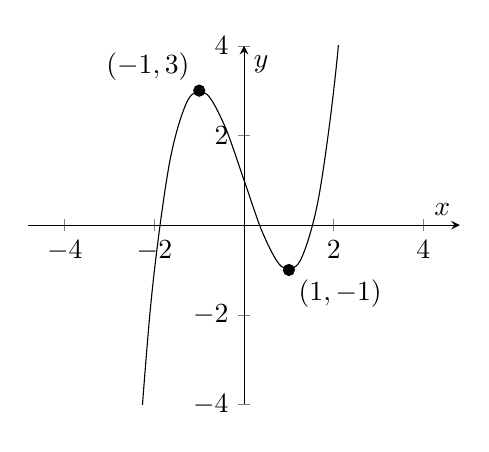
\begin{tikzpicture}[cmark/.style={label={[anchor=center]:\pgfuseplotmark{#1}}}]
			\begin{axis}
			[
				restrict y to domain=-10:10,
				restrict x to domain=-5:5,
				xlabel=$x$,
				ylabel=$y$,
				xmin=-4,
				xmax=4,
				xtick={-4,-2,...,4},
				ymin=-4,
				ymax=4,
				ytick={-4,-2,...,3},
				axis lines=center,
				axis equal,
				smooth,
				scale=0.8
			]
			\addplot [] {x^3-3*x+1};
			\coordinate
			[
				label=above left:{$(-1,3)$},
				black,
				cmark=*,
			] (a) at (-1,3);
			\coordinate
			[
				label=below right:{$(1,-1)$},
				black,
				cmark=*,
			] (a) at (1,-1);
			\end{axis}
		\end{tikzpicture}
		\caption{Some function $y=f(x)$ with a couple of given coordinates.}
	\end{subfigure}
	\begin{subfigure}{0.475\linewidth}
		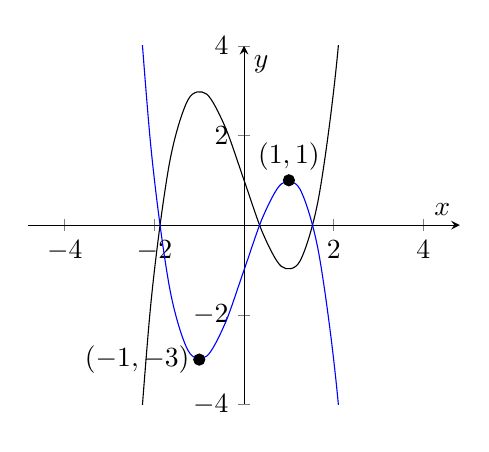
\begin{tikzpicture}[cmark/.style={label={[anchor=center]:\pgfuseplotmark{#1}}}]
			\begin{axis}
			[
				restrict y to domain=-10:10,
				restrict x to domain=-5:5,
				xlabel=$x$,
				ylabel=$y$,
				xmin=-4,
				xmax=4,
				xtick={-4,-2,...,4},
				ymin=-4,
				ymax=4,
				ytick={-4,-2,...,3},
				axis lines=center,
				axis equal,
				smooth,
				scale=0.8
			]
			\addplot [mark=none] {x^3-3*x+1};
			\addplot [color=blue,mark=none] {-x^3+3*x-1};
			\coordinate
			[
				label=left:{$(-1,-3)$},
				black,
				cmark=*,
			] (a) at (-1,-3);
			\coordinate
			[
				label=above:{$(1,1)$},
				black,
				cmark=*,
			] (a) at (1,1);
			\end{axis}
		\end{tikzpicture}
		\caption{$y=-f(x)$ in blue, along with the original graph.}
	\end{subfigure}
	\caption{An example of a typical question about $y=-f(x)$ with the solution.}
	\label{fig:xAxisReflectionExample}
\end{figure}

To find out the transformed coordinates, change the $y$-coordinates' sign:
\begin{align*}
	f(x)&=(-1,3) & f(x)&=(1,-1)\\
	-f(x)&=(-1,-3) & -f(x)&=(-1,-1)
\end{align*}


\section{Graph of $y=f(-x)$}
$y=f(-x)$ is reflection on the y-axis; all $x$-coordinates will change their signs.

\subsection{Example}
Here in figure \ref{fig:yAxisReflectionExample} an example of reflection on the $y$-axis is shown with the coordinates $(1,2)$ and $(3,-2)$.

\begin{figure}[h!]
	\centering
	\begin{subfigure}{0.475\linewidth}
		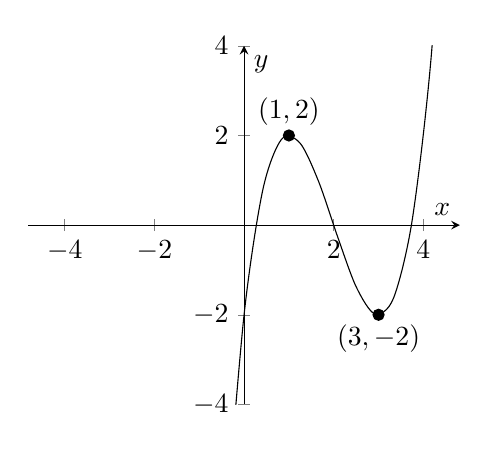
\begin{tikzpicture}[cmark/.style={label={[anchor=center]:\pgfuseplotmark{#1}}}]
			\begin{axis}
			[
				restrict y to domain=-10:10,
				restrict x to domain=-5:5,
				xlabel=$x$,
				ylabel=$y$,
				xmin=-4,
				xmax=4,
				xtick={-4,-2,...,4},
				ymin=-4,
				ymax=4,
				ytick={-4,-2,...,3},
				axis lines=center,
				axis equal,
				smooth,
				scale=0.8
			]
			\addplot [] {(x-2)^3-3*x+6};
			\coordinate
			[
				label=above:{$(1,2)$},
				black,
				cmark=*,
			] (a) at (1,2);
			\coordinate
			[
				label=below:{$(3,-2)$},
				black,
				cmark=*,
			] (a) at (3,-2);
			\end{axis}
		\end{tikzpicture}
		\caption{Some function $y=f(x)$ with a couple of given coordinates.}
	\end{subfigure}
	\begin{subfigure}{0.475\linewidth}
		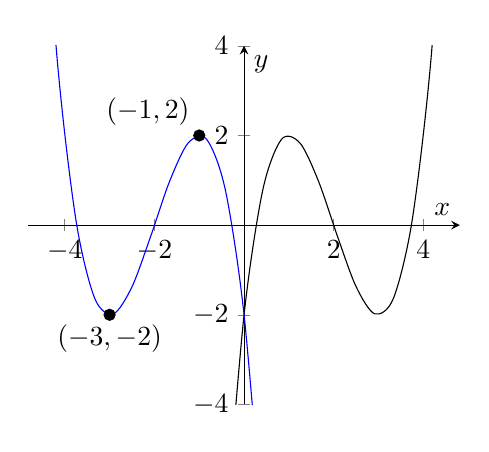
\begin{tikzpicture}[cmark/.style={label={[anchor=center]:\pgfuseplotmark{#1}}}]
			\begin{axis}
			[
				restrict y to domain=-10:10,
				restrict x to domain=-5:5,
				xlabel=$x$,
				ylabel=$y$,
				xmin=-4,
				xmax=4,
				xtick={-4,-2,...,4},
				ymin=-4,
				ymax=4,
				ytick={-4,-2,...,3},
				axis lines=center,
				axis equal,
				smooth,
				scale=0.8
			]
			\addplot [mark=none] {(x-2)^3-3*x+6};
			\addplot [color=blue,mark=none] {(-x-2)^3+3*x+6};
			\coordinate
			[
				label=above left:{$(-1,2)$},
				black,
				cmark=*,
			] (a) at (-1,2);
			\coordinate
			[
				label=below:{$(-3,-2)$},
				black,
				cmark=*,
			] (a) at (-3,-2);
			\end{axis}
		\end{tikzpicture}
		\caption{$y=f(-x)$ in blue, along with the original graph.}
	\end{subfigure}
	\caption{An example of a typical question about $y=f(-x)$ with the solution.}
	\label{fig:yAxisReflectionExample}
\end{figure}

To find out the transformed coordinates, change the $x$-coordinates' sign:
\begin{align*}
	f(x)&=(1,2) & f(x)&=(3,-2)\\
	f(-x)&=(-1,2) & f(-x)&=(-3,-2)
\end{align*}


\section{Graph of $y=kf(x)$}
A graph can be stretched or compressed on the $y$-axis by multiplying the graph by a constant, written as $y=kf(x)$. $k>1$ will stretch it, while $k<1$ will compress it.

To find out the new coordinates, multiply the $y$-coordinate by $k$.

\subsection{Example}
Figure \ref{fig:verticalCompressionExample} is the graph of $y=f(x)$, as well as $y=2f(x)$ and $y=\frac{1}{2}f(x)$.

\begin{figure}[h!]
	\centering
	\begin{subfigure}{0.475\linewidth}
		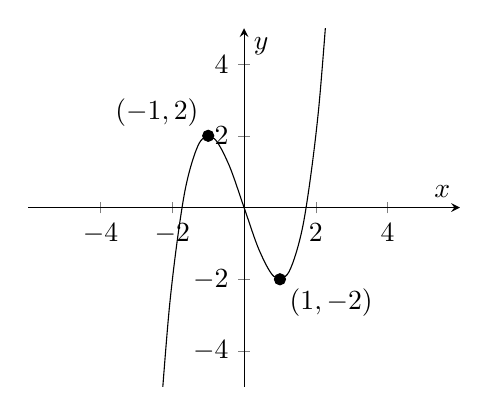
\begin{tikzpicture}[cmark/.style={label={[anchor=center]:\pgfuseplotmark{#1}}}]
			\begin{axis}
			[
				restrict y to domain=-10:10,
				restrict x to domain=-5:5,
				xlabel=$x$,
				ylabel=$y$,
				xmin=-5,
				xmax=5,
				xtick={-4,-2,...,4},
				ymin=-5,
				ymax=5,
				ytick={-4,-2,...,4},
				axis lines=center,
				axis equal,
				smooth,
				scale=0.8,
			]
			\addplot [] {x^3-3*x};
			\coordinate
			[
				label=above left:{$(-1,2)$},
				black,
				cmark=*,
			] (a) at (-1,2);
			\coordinate
			[
				label=below right:{$(1,-2)$},
				black,
				cmark=*,
			] (a) at (1,-2);
			\end{axis}
		\end{tikzpicture}
		\caption{Some function $y=f(x)$ with a couple of given coordinates.}
	\end{subfigure}
	\begin{subfigure}{0.475\linewidth}
		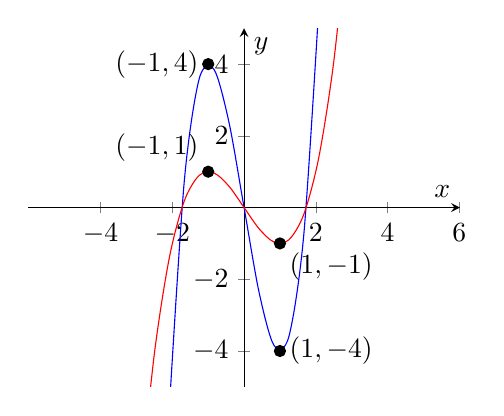
\begin{tikzpicture}[cmark/.style={label={[anchor=center]:\pgfuseplotmark{#1}}}]
			\begin{axis}
			[
				restrict y to domain=-10:10,
				restrict x to domain=-5:5,
				xlabel=$x$,
				ylabel=$y$,
				xmin=-5,
				xmax=5,
				xtick={-4,-2,...,5},
				ymin=-5,
				ymax=5,
				ytick={-4,-2,...,4},
				axis lines=center,
				axis equal,
				smooth,
				scale=0.8,
			]
			\addplot [color=blue,mark=none] {2*(x^3)-6*x};
			\addplot [color=red,mark=none] {0.5*(x^3)-1.5*x};
			\coordinate
			[
				label=left:{$(-1,4)$},
				black,
				cmark=*,
			] (a) at (-1,4);
			\coordinate
				[
				label=right:{$(1,-4)$},
				black,
				cmark=*,
			] (a) at (1,-4);
			\coordinate
			[
				label=above left:{$(-1,1)$},
				black,
				cmark=*,
			] (a) at (-1,1);
			\coordinate
			[
				label=below right:{$(1,-1)$},
				black,
				cmark=*,
			] (a) at (1,-1);
			\end{axis}
		\end{tikzpicture}
		\caption{$y=2f(x)$ in blue and $y=\frac{1}{2}f(x)$, original graph omitted for clarity.}
	\end{subfigure}
	\caption{An example of a typical question about $y=kf(x)$ with the solution.}
	\label{fig:verticalCompressionExample}
\end{figure}

To find out the transformed coordinates, multiply the $y$-coordinates by $k$. For $k=2$:
\begin{align*}
f(x)&=(-1,2) & f(x)&=(1,-2)\\
f(2x)&=(-1,4) & f(2x)&=(1,-4)
\end{align*}
And for $k=\frac{1}{2}$:
\begin{align*}
f(x)&=(-1,2) & f(x)&=(1,-2)\\
f\left(\frac{1}{2}x\right)&=(-1,1) & f\left(\frac{1}{2}x\right)&=(1,-1)
\end{align*}


\section{Graph of $y=f(kx)$}
The last transformation is stretching and compressing on the $x$-axis. Again, the opposite is true here, $k>1$ will \textit{compress} the graph, $k<1$ will stretch the graph.

To get the new coordinates, divide all $x$-coordinates by $k$.

\subsection{Examples}
Figure \ref{fig:horizontalCompressionExample} shows $y=f(x)$, and the graphs of $y=f(2x)$ and $y=f(\frac{1}{2})$.

\begin{figure}[h!]
	\centering
	\begin{subfigure}{0.475\linewidth}
		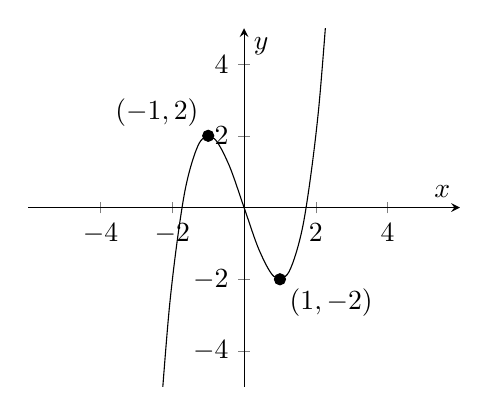
\begin{tikzpicture}[cmark/.style={label={[anchor=center]:\pgfuseplotmark{#1}}}]
			\begin{axis}
			[
				restrict y to domain=-10:10,
				restrict x to domain=-5:5,
				xlabel=$x$,
				ylabel=$y$,
				xmin=-5,
				xmax=5,
				xtick={-4,-2,...,4},
				ymin=-5,
				ymax=5,
				ytick={-4,-2,...,4},
				axis lines=center,
				axis equal,
				smooth,
				scale=0.8,
			]
			\addplot [] {x^3-3*x};
			\coordinate
			[
				label=above left:{$(-1,2)$},
				black,
				cmark=*,
			] (a) at (-1,2);
			\coordinate
			[
				label=below right:{$(1,-2)$},
				black,
				cmark=*,
			] (a) at (1,-2);
			\end{axis}
		\end{tikzpicture}
		\caption{Some function $y=f(x)$ with a couple of given coordinates.}
	\end{subfigure}
	\begin{subfigure}{0.475\linewidth}
		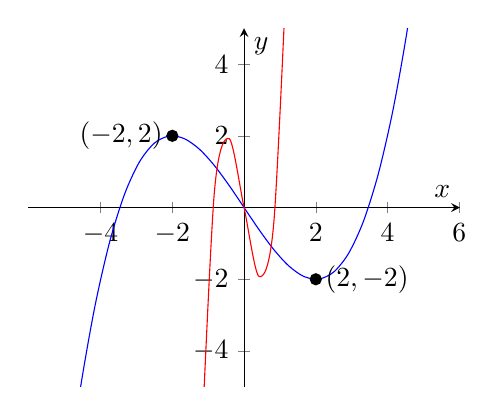
\begin{tikzpicture}[cmark/.style={label={[anchor=center]:\pgfuseplotmark{#1}}}]
			\begin{axis}
			[
				restrict y to domain=-10:10,
				restrict x to domain=-5:5,
				xlabel=$x$,
				ylabel=$y$,
				xmin=-5,
				xmax=5,
				xtick={-4,-2,...,5},
				ymin=-5,
				ymax=5,
				ytick={-4,-2,...,4},
				axis lines=center,
				axis equal,
				smooth,
				scale=0.8,
			]
			\addplot [color=blue,mark=none] {(x/2)^3-1.5*x};
			\addplot [color=red,mark=none] {(2*x)^3-6*x};
			\coordinate
			[
				label=left:{$(-2,2)$},
				black,
				cmark=*,
				] (a) at (-2,2);
			\coordinate
			[
				label=right:{$(2,-2)$},
				black,
				cmark=*,
			] (a) at (2,-2);
			\end{axis}
		\end{tikzpicture}
		\caption{$y=f(\frac{1}{2}x)$ in blue and $y=f(2x)$ in red, original graph and coordinates of $y=f(\frac{1}{2}x)$ omitted for clarity.}
	\end{subfigure}
	\caption{An example of a typical question about $y=f(kx)$ with the solution.}
	\label{fig:horizontalCompressionExample}
\end{figure}

To find out the transformed coordinates, divide the $x$-coordinates by $k$. For $k=\frac{1}{2}$:
\begin{align*}
f(x)&=(-1,2) & f(x)&=(1,-2)\\
f(2x)&=(-2,2) & f(2x)&=(2,-2)
\end{align*}
And for $k=2$:
\begin{align*}
f(x)&=(-1,2) & f(x)&=(1,-2)\\
f\left(\frac{1}{2}x\right)&=\left(-\frac{1}{2},2\right) & f\left(\frac{1}{2}x\right)&=\left(\frac{1}{2},-1\right)
\end{align*}